\documentclass{standalone}
\usepackage{amsmath}
\usepackage[T1]{fontenc}
\usepackage[utf8]{inputenc}

\usepackage[usenames,dvipsnames]{xcolor}

\usepackage{tikz}
\usetikzlibrary{arrows, shapes, matrix}

\begin{document}

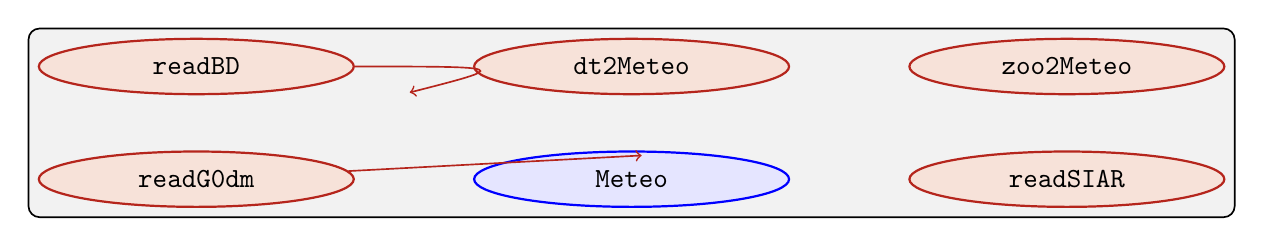
\begin{tikzpicture}[auto,
  function/.style ={draw=BrickRed, thick, ellipse, fill=BrickRed!10,
    minimum height=2em},
  % 
  class/.style ={draw=Blue, thick, ellipse, fill=Blue!10,
    minimum height=2em} ]
  
  \tikzset{every path/.style={line width=.6pt}}

  \begin{scope}
    \matrix [matrix of nodes, rounded corners, fill=gray!10, draw=black, column
  sep=15mm,row sep=7mm, minimum width=4cm] (Meteo) {
    %%%%%%%%%%%%%%%%%%%%%%%%%%%%%%% 
    \node [function](readBD){\texttt{readBD}}; &
    \node [function](dt2Meteo){\texttt{dt2Meteo}}; &
    \node [function](zoo2Meteo){\texttt{zoo2Meteo}}; \\
    %%%%%%%%%%%%%%%%%%%%%%%%%%%%%%%
    \node [function](readG0dm){\texttt{readG0dm}}; &
    \node [class](Meteo){\texttt{Meteo}}; &
    \node [function](readSIAR){\texttt{readSIAR}}; \\
  };
\end{scope}

\begin{scope}
  \draw [->, BrickRed] (readG0dm) -- (Meteo);
  \draw [->, BrickRed] (readBD) .. controls ++(0:4) .. (Meteo);
  % \draw [->, Green] (eo) .. controls ++(0:4) .. (fSolD)
  % node [midway, above, simple] {$\epsilon_o$};
  % \draw [->, Green] (EoT) -- (fSolD)
  % node [midway, above, simple] {$EoT$};
  % \draw [->, Green] (ws) .. controls ++(0:4) .. (fSolD)
  % node [midway, above, simple] {$\omega_s$};
  % \draw [->, Green] (Bo0d) .. controls ++(0:4) .. (fSolD)
  % node [midway, above, simple] {$B_{0d}(0)$};
  % \draw [->, Green] (w) .. controls ++(0:-4) .. (fSolI)
  % node [midway, above, simple] {$\omega$};
  % \draw [->, Green] (cosThzS) -- (fSolI)
  % node [midway, above, simple] {$cos(\theta_{zs})$};
  % \draw [->, Green] (AzS) .. controls ++(0:-4) .. (fSolI)
  % node [midway, above, simple] {$\psi_s$};
  
\end{scope}
  
\end{tikzpicture}

\end{document}
